\section{Theory}
%TODO: Need theory about ccd? It is not really relevant is it?
%Need theory about the different uses of the same sensor in spectrometer and camera, I need this defend that the values should have an correlation. 

\subsection{Camera}
Cameras are widely used to photograph objects, and works by focusing light onto a photo-sensor. The camera used in this thesis uses a Charged-coupled device (CCD) photo-sensor \cite{JYIVolumeThree}.

\subsection{Spectrometry}
Spectrometer is a widely used tool for analyzing substances. It is a remote sensing tool that give good spectral information about the light that enters the fiber. As can be seen in figure \ref{fig:spectrometer_inside} the light is split into the different wavelengths before hitting the CCD sensor. This has the effect that the sensor reads spectral information instead of spatial as a camera would. 

\begin{figure}[h]
    \centering
    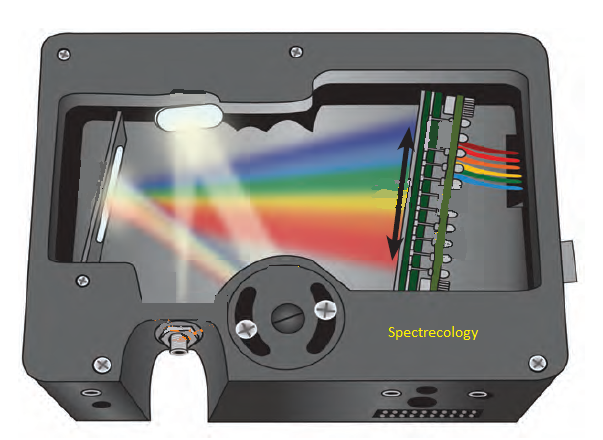
\includegraphics[width=0.5\textwidth]{figures/Mini-spectrometer-open-bench.png}
    \caption{Inside of a spectrometer \cite{KAI0340640480}}
    \label{fig:spectrometer_inside}
\end{figure}

Because of this it can be used to give an average spectrum of the area under the acceptance cone of the fiber. 
%TODO3 Add theory about how the spectrometer works. I could maybe skip this point as it is not necessary for explaining the correlation, but I'm afraid it is necessary for a rigorous description of why the correlation makes sense. Same for the camera

\subsection{Reflection}
\label{sec:theory_reflection}
Reflection of light describes the notion of light hitting materials and getting a change of path due to the exchange of energy with the material. There are two extremes when we talk about reflection:

\textbf{Specular reflection} denotes the case where the light is reflected in a unison manner from the sample, all in one direction. This concept is shown in figure \ref{fig:specular_reflection}.

\begin{figure}[h!]
    \centering
    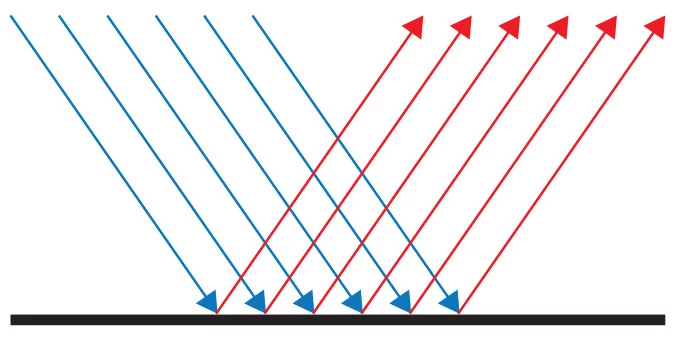
\includegraphics[width=0.5\textwidth]{figures/theory/Specular-Reflection.png}
    \caption{Example of specular reflection \cite{SpecularReflectionOcean}}
    \label{fig:specular_reflection}
\end{figure}

\textbf{Diffusive reflection} denotes the case where the light is scattered in every direction. This concept is shown in figure \ref{fig:diffusive_reflection}.

\begin{figure}[h!]
    \centering
    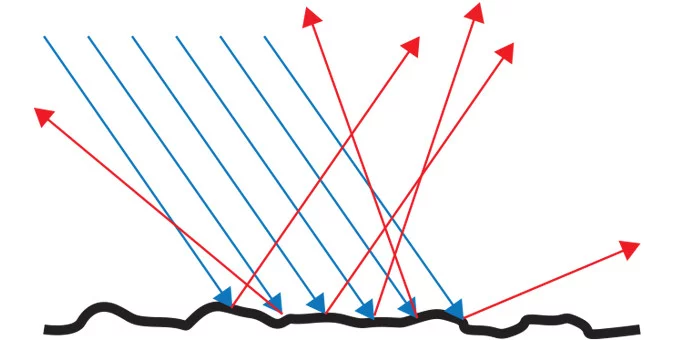
\includegraphics[width=0.5\textwidth]{figures/theory/Diffuse-Reflection.png}
    \caption{Example of diffusive reflection \cite{DiffuseReflectionOcean}}
    \label{fig:diffusive_reflection}
\end{figure}

Both of these reflection types are ideal and all real reflection will be a combination of these two. Not even the best available mirrors exhibit perfect specular properties, and no material scatters light equally in all directions. It is however useful to have two extremes to compare the results too. 

%TODO: Im not sure yet about including these
%\subsubsection{Specular} 
%\subsubsection{Diffusive}
%\subsection{Relative reflection}

\subsection{Noise and dark current}
\label{sec:noise_and_dark_current}
Both the images and the spectrums will have noise in them, making the readings less accurate. One type of noise that is a problem in spectrometry is noise from dark currents. These are currents that will be detected in the CCD sensor even though there is no incoming light. 



%TODO: Should add:
% Linear regression
% Colorimetry
% 